\chapter{Generowanie wykresów}

Wykresy powinny być wykonane starannie, z zachowaniem odpowiedniej czytelności. Należy zatem generować je w wyspecjalizowanym do tego celu programie i zapisywać do pliku w formacie grafiki wektorowej. Proponuje się w tym celu program \texttt{GNU Octave} lub \texttt{gnuplot}. Odpowiednio wykonany rysunek powinien cechować się identycznym krojem i wielkością czcionki, co osiągnięto w przypadku rysunku~\ref{fig:octave}, stosując przykładowy skrypt~\ref{lst:octave}.

\begin{figure}[htb!]
\centering
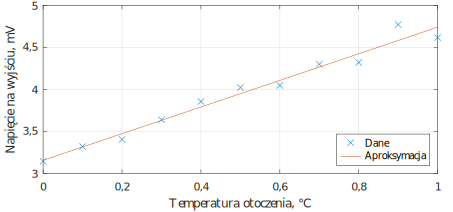
\includegraphics{plot_demo}
\makecaption{fig:octave}{Przykładowy rysunek wygenerowany w programie \texttt{GNU Octave}}
\end{figure}

\begin{listing}[hbt!]
\inputminted[linenos, breaklines]{octave}{skrypty/plot_demo.m}
\makecaption{lst:octave}{Przykładowy skrypt programu \texttt{GNU Octave} generujący rysunek~\ref{fig:octave}}
\end{listing}

Przedstawiony skrypt tworzy w pierwszej linii nowy wykres, przy czym gdy skrypt zostaje wywołany z terminala wykres ten jest ukrywany (taki zabieg ułatwia wsadowe generowanie wykresów). Następnie ustalane są wymiary wykresu (linie 5--7) oraz korygowana jest jego pozycja tak, aby wypełniał on cały obszar rysunku (linia 10). W kolejnych liniach (12--16) ustalane są parametry czcionki, przy czym z nieznanych dla autora niniejszego szablonu powodów, dla rozmiaru \qty{11}{pt} wynikowy plik cechuje się czcionką o rozmiarze \qty{12}{pt} (najprawdopodobniej występuje błąd w programie \texttt{GNU Octave}, związany ze skalowaniem obrazu).

Po wygenerowaniu danych wykres jest sporządzany oraz formatowane są jego elementy. W opisach stosować można większość podstawowych funkcji \LaTeX{} do formatowania tekstu. Można również zastosować wartość \texttt{'latex'} dla opcji \texttt{'interpreter'} formatując kolejne elementy wykresu. Szczegóły opisuje \href{https://docs.octave.org/latest}{dokumentacja} programu \texttt{GNU Octave}. Znaki specjalne wstawiać można bezpośrednio w edytorze tekstu, stosując kodowanie \texttt{UTF-8}. Można także wstawiać je stosując ich nazwy, identycznie jak podczas edycji równań. Wygenerowany w omawiany sposób wykres jest spójny z resztą dokumentu i wygląda profesjonalnie. Niestety, stosowanie \LaTeX{} w programie \texttt{GNU Octave} jest mocno ograniczone.

Wykresy można generować również w programie \texttt{gnuplot}, gdzie przykładowy skrypt przedstawiono w listingu~\ref{lst:gnuplot}. Stosować w tym celu można terminal \texttt{tikz}, który umożliwia wygenerowanie skryptu \LaTeX{} gotowego do osadzenia w dokumencie. Zauważyć można, że tytuł wykresu \enquote{$f(x) = e^{-0.1x} \cdot \sin(x)$} z rysunku~\ref{fig:gnuplot} wygląda identycznie, jak w tekście.

\begin{figure}[htb!]
\centering
\includegraphics{gnuplot_demo}
\makecaption{fig:gnuplot}{Przykładowy rysunek wygenerowany w programie \texttt{gnuplot}}
\end{figure}

\begin{listing}[hbt!]
\inputminted[linenos, breaklines]{gnuplot}{skrypty/plot_demo.gnuplot}
\makecaption{lst:gnuplot}{Przykładowy skrypt programu \texttt{gnuplot} generujący rysunek~\ref{fig:gnuplot}}
\end{listing}

Ostatnim proponowanym rozwiązaniem jest ręczne generowanie wykresów bezpośrednio w treści dokumentu, stosując bibliotekę \texttt{pgfplots} oraz środowisko \texttt{tikzpicture}. Takie rozwiązanie zapewnia jakość porównywalną do stosowania programu \texttt{gnuplot} i terminala \texttt{tikz}, przy czym wymaga wprowadzenia treści wykresu ręcznie. Przykład wykresu, który generowany jest na podstawie listingu~\ref{lst:pgfplots} przedstawia rysunek~\ref{fig:pgfplots}, przy czym osiągnięty efekt jest podobny do rysunku~\ref{fig:gnuplot}.

\begin{figure}[htb!]
\centering
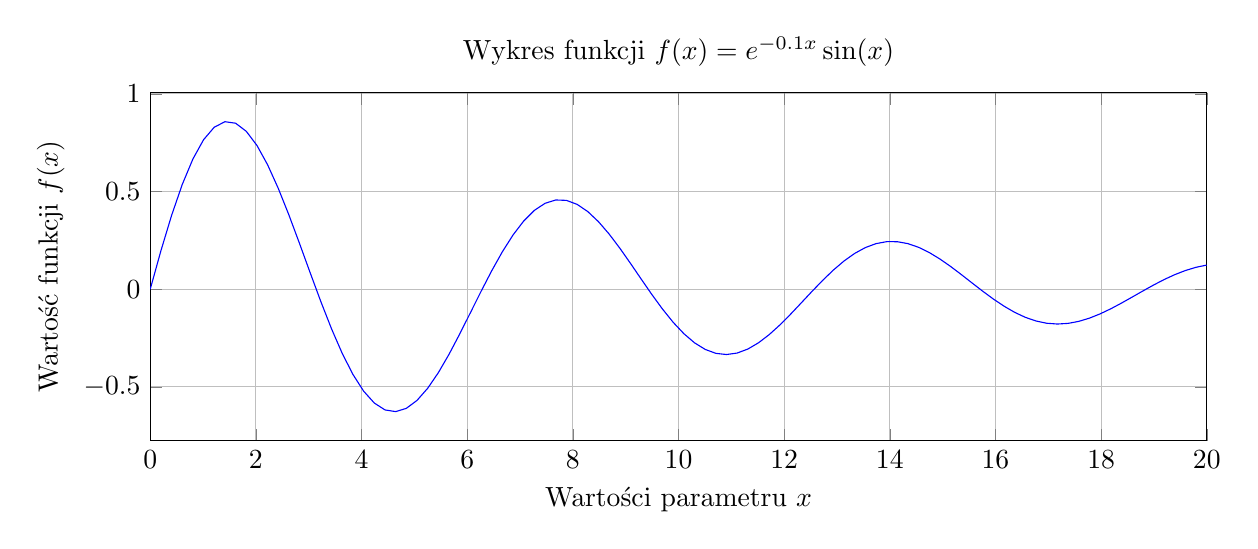
\begin{tikzpicture}
	\begin{axis}[
		title = {Wykres funkcji $f(x) = e^{-0.1x} \sin(x)$},
		xlabel = {Wartości parametru $x$},  % opis osi X
		ylabel = {Wartość funkcji $f(x)$},  % opis osi Y
		width = 15cm, height = 6cm,         % wymiary wykresu
		xmin = 0, xmax = 20,                % ograniczenia osi X
		grid = both,                        % siatka pomocnicza
	]
	\addplot[blue, domain = 0:20, samples = 100]{ exp(-0.1*x)*sin(deg(x)) };
	\end{axis}
\end{tikzpicture}
\makecaption{fig:pgfplots}{Przykładowy rysunek wygenerowany w bibliotece \texttt{pgfplots}}
\end{figure}

\begin{listing}[ht!]
\begin{minted}[linenos, breaklines]{latex}
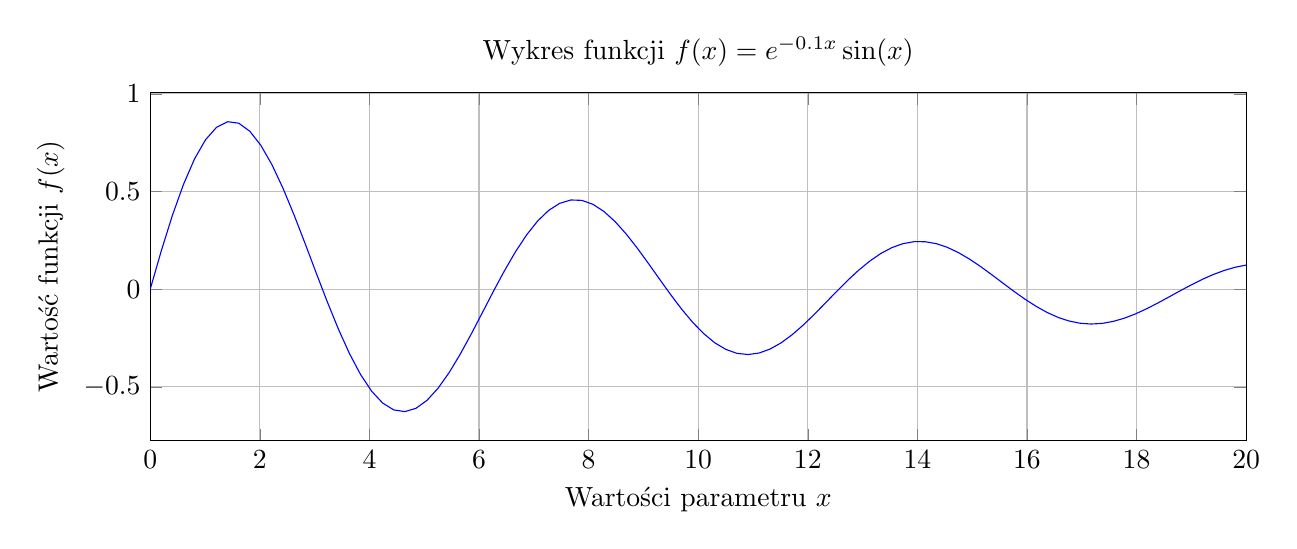
\begin{tikzpicture}
	\begin{axis}[
		title = {Wykres funkcji $f(x) = e^{-0.1x} \sin(x)$},
		xlabel = {Wartości parametru $x$},  % opis osi X
		ylabel = {Wartość funkcji $f(x)$},  % opis osi Y
		width = 15.5cm, height = 6cm,       % wymiary wykresu
		xmin = 0, xmax = 20,                % ograniczenia osi X
		grid = both,                        % siatka pomocnicza
	]
	\addplot[blue, domain = 0:20, samples = 100]
		{ exp(-0.1*x)*sin(deg(x)) };
	\end{axis}
\end{tikzpicture}
\end{minted}
\makecaption{lst:pgfplots}{Przykładowy wykres wygenerowany w bibliotece \texttt{pgfplots}}
\end{listing}

Generowanie wykresów w programie \texttt{GNU Octave} jest najprostszym z przedstawionych rozwiązań, gdzie dodatkowo program ten pozwala na przeprowadzanie skomplikowanych symulacji i obliczeń. Program \texttt{gnuplot} umożliwia natomiast generowanie wykresów dużo lepszej jakości, gdzie jednocześnie możliwe jest wykonywanie różnych operacji i obliczeń na danych, które mogą być wczytywane z plików. Stosowanie biblioteki \texttt{pgfplots} zapewnia doskonałą jakość wykresów i grafów, natomiast wymaga wprowadzania ich bezpośrednio w kodzie \LaTeX{} lub wczytywania treści skryptu z pliku. Dobór stosowanego rozwiązania powinien być zatem rozważony pod kątem łatwości użycia danego narzędzia oraz zapewnianych przez niego możliwości. Istotne jest jednak, aby wszystkie wykresy w pracy były jednolite -- najlepiej zatem stosować konsekwentnie jedno z rozwiązań.
